\documentclass{report}
\usepackage[pdftex]{graphicx}
\usepackage{sidecap}
\usepackage{fancyhdr}
\usepackage{lscape}
\usepackage[francais]{babel} 
\usepackage[absolute]{textpos}
\usepackage{amssymb}

\usepackage{siunitx}
\usepackage[utf8]{inputenc}  
\usepackage[T1]{fontenc}


\title{Rapport de labo d'\'electronique: \\ Etude des caractéristiques d'un transistor BJT}
\author{Groupe ?: \\ Mattens Simon; Dom Eduardo \\ BA2 Info}
\date{Labo r\'ealis\'e le 9 mai 2018}

\pagestyle{fancy}
\lhead{Groupe ?: Mattens S. ; Dom E.}
\rhead{BA2 Info}
\cfoot{\thepage}
\begin{document}
\maketitle

\section*{1. Introduction}
Le but de la manipulation est l'étude détaillée des caractéristiques électriques d'un transistor bipolaire à jonction.

\section*{2. R\'esum\'e th\'eorie}
\begin{itemize}
\item Un transistor BJT est un monocristal comprenant 3 régions : 2 régions p séparées par une région n ou 2 régions n séparées par une région p. (Transistor npn ou pnp). On y trouve 2 diodes de telle sorte que la région n ou p soit commune aux 2 diodes les 3 lettres désignant la succession des 3 types constituant le monocristal.\\
On appelle Base la région commune p (ou n); émettur la région n( ou p) de la diode 1, collecteur la région n( ou p) de la diode 2. Voici un schéma d'un transisor Pnp et Npn :
\begin{figure}[h!]
\centering
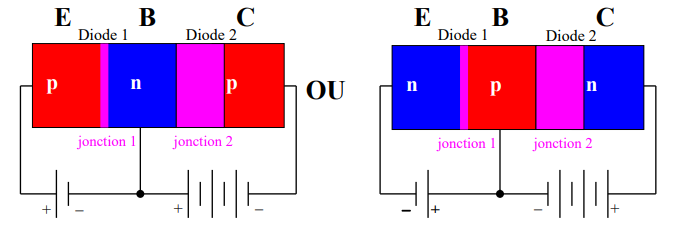
\includegraphics[scale=0.5]{Trans.png}
\end{figure}

\item Ie=Ib+Ic : le courant Ib(base) est très petit comparé au courant Ic(collecteur) et au courant Ie(émetteur). On pose généralement  Ic=$\alpha$Ie. Le coefficient $\alpha$, proche de l'unité, donnant la fraction des porteurs de charge injectés par l'émetteur dans la base qui sortent par le collecteur.
\\On pose Ic=$\beta$Ib où $\beta$ est le coefficient d'amplification ou gain en courant du transistor.
\item A une faible variation $\Delta$Ib du courant Ib correspond une variation importante $\Delta$Ic du courant Ic; c'est l'effet physique mis en oeuvre dans un transistor utilisé comme amplificteur:
\begin{figure}[h!]
\centering
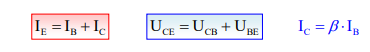
\includegraphics[scale=1]{Amp1.png}
\end{figure}
\newpage
\item Jonction E-B (polarisée en sens direct): caractéristique courant - tension ou courbe Ib=f(Ube) avec paramètre Uce. On observera l'allure de la courbe "diode" polarisée en sens passant : Ib nul jusqu'à un seuil, coude, puis Ib augmente linéairement avec U :
\begin{figure}[h!]
\centering
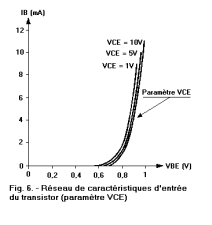
\includegraphics[scale=0.5]{Amp2.png}
\end{figure}
\item Jonction B-c (polarisée en sens inverse): caractéristique courant - tension ou courbe Ic=f(Uce) avec paramètre Ib. La valeur du paramètre Ib influence fortement le fonctionnement du transistor.Aux faiblesvaleurs Uce: comportement ohmique,coude puis aux valeurs Uce plus élevées : Ic quasi constant qu'elle que soit la valeur de Ib :
\begin{figure}[h!]
\centering
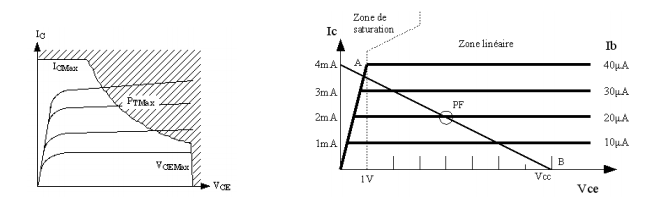
\includegraphics[scale=0.5]{Amp3.png}
\end{figure}
\item U=U0(Rcb/Rtot)
\end{itemize}

\section*{3 Dispositif expérimental}

\begin{itemize}
\item Transistor étudiée : Il s'agit d'un transistor BJT de modèle 2N1711.
\begin{figure}[h!]
\centering
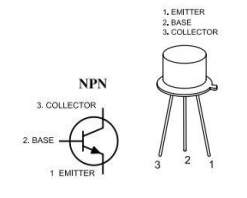
\includegraphics[scale=0.5]{Man1.png}
\end{figure}
\newpage
\item Polarisation du Transistor : Montage en émetteur commun. L'émetteur est à la masse et les résistances Rb et Rc sont à choisir pour définir la polarisation, suivant l'étude à effectuer. On utilise une source de tension continue (0-30V) que l'on fixe à E=9V.
\begin{figure}[h!]
\centering
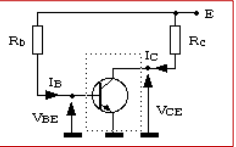
\includegraphics[scale=0.5]{Man2.png}
\end{figure}
\item Pour les prises de mesures de courant ou de différence de potentiel, nous utiliserons des multimètres digitaux ainsi qu'un microampèremètre à aiguille ou un multimètre digital ITC 921 pour pouvoir mesurer des "petits" courants.\\
Pour tester le principe d'amplification des signaux alternatifs, on utilisera un générateur de signaux pour générer le signal d'entrée et un oscilloscope pour mesurer les signaux d'entrée et de sortie.\\
\end{itemize}
Il nous ait demandé de monter les circuits suivants : \\\\
\textbf{Circuit 1 : }
\begin{figure}[h!]
\centering
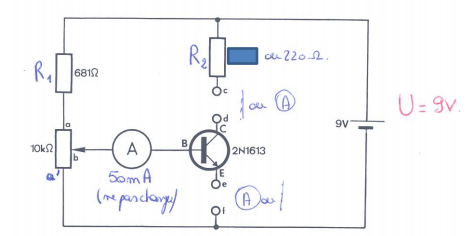
\includegraphics[scale=0.5]{Cir1.png}
\end{figure}

\textbf{Circuit 2: }
\begin{figure}[h!]
\centering
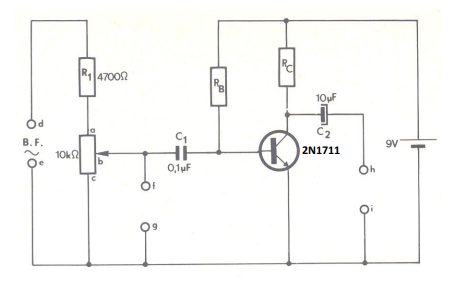
\includegraphics[scale=0.5]{Cir2.png}
\end{figure}



\section*{4 Prise des mesures et résultats}


\subsection*{4.1 Préambule : utilisataion d'un potentiomètre}
Potentiomètre = 10,4k$\si{\ohm}$\\
Quand je mesure la résistance entre la borne du milieu et une borne extrême du potentiomètre j'obtiens la valeur : 8,2k$\si{\ohm}$. Et quand je mesure la borne du milieur avec l'autre extrême j'ai la valeur : 2,2k$\si{\ohm}$.


\subsection*{4.2 Vérification de la relation liant les trois courants}
(Nous utilisons le circuit 1 présent dans la section Dispositif expérimental).
\textbf{\'Enonc\'e:} En faisant varier le potentiomètre, relever plusieurs points Ib,Ic,Ie afin de vérifier la relation Ie=Ib+Ic. \\

\textbf{R\'eponse:} \\
Ie=10,4k$\si{\ohm}$ \  Ib=8,2k$\si{\ohm}$ \ Ic=2,2k$\si{\ohm}$\\
Ie=10,4k$\si{\ohm}$  \ Ib=6,4k$\si{\ohm}$  \ Ic=4k$\si{\ohm}$\\
Ie=10,4k$\si{\ohm}$ \  Ib=3k$\si{\ohm}$ \  Ic=7,4k$\si{\ohm}$

\subsection*{4.3 Etude de la variation Ic=f(Ib) et gain en courant Ic=$\beta$Ib}
(Nous utilisons le circuit 1 présent dans la section Dispositif expérimental).
\begin{tabular}{|c|c|}
\hline
\textbf{Courant de Base Ib($\mu$A)} & \textbf{Courant de collecteur Ic(mA)}  \\
\hline
49 & 4  \\
\hline
74,5 & 11 \\
\hline
91,3 & 14 \\
\hline
119,2 & 19 \\
\hline
137,5 & 21 \\
\hline
177 & 27 \\
\hline
210 & 32  \\
\hline
240 & 35\\
\hline
276 & 37\\
\hline
336 & 37\\
\hline
442 & 37\\
\hline
\end{tabular}
\newpage
\textbf{\'Enonc\'e:} Tracer un graphique Ic=f(Ib) et déterminer le gain courant du transistor comme pente de la droite \\

\textbf{R\'eponse:} \\
\begin{figure}[h!]
\centering
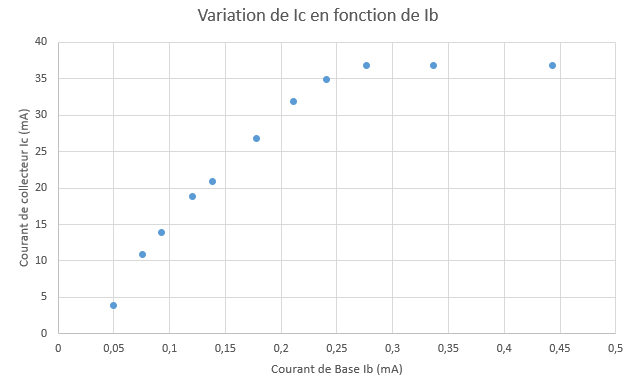
\includegraphics[scale=0.5]{Graphe.png}
\end{figure}

La pente de la droite a été calculée avec Excel. Elle vaut 157mA.


\textbf{\'Enonc\'e:} Pour comparaison, mesurer également le gain en courant au moen d'un multimètre en utilisant la borne multifonctionnelle\\

\textbf{R\'eponse:} \\
$\beta$=162mA

\subsection*{4.5 Utilisation du transistor en amplificateur (à 1 étage) : amplification de signaux alternatifs sinusoidaux}
(Nous utilisons le circuit 2 présent dans la section Dispositif expérimental).
\\
\\
\begin{tabular}{|c|c|c|}
\hline
\textbf{Fréquence(Hz)} & \textbf{Amplitude Vin (mV)} & \textbf{Vout(V)} \\
\hline
170 & 227 & 1,72  \\
\hline
400 & 180 & 3,07 \\
\hline
750 & 118 & 3,61 \\
\hline
1100 & 90 & 3,76 \\
\hline
\end{tabular}


\section*{5 Analyse des résultats}
\subsection*{5.2 Vérification de la relation liant les trois courants}
Nous remarquons que l'équation Ie=Ib+Ic est toujours vérifiée. En effet nous arrivons toujours à Ie=10,4k$\si{\ohm}$.
Quand on actionne dans un sens le curseur du potentiomètre avec un tournevis, la résitance de Ib diminue(et celle de Ic augmente) et dans l'autre sens la résistance de Ib augmente et celle de Ic diminue (Ie reste à 10,4k$\si{\ohm}$.)
\subsection*{5.3 Etude de la variation Ic=f(Ib) et gain en courant Ic=$\beta$Ib}
Nous remarquons qu'à partir d'un certain seuil de Ic (ici le seuil est à 37 $\mu$A), Ic reste constant tandis que Ib continue à croître.
\subsection*{5.5 Utilisation du transistor en amplificateur (à 1 étage) : amplification de signaux alternatifs sinusoidaux}
Au plus la fréquence augmente et Vin diminue au plus Vout augmente.

\section*{6 Conclusion}

Durant cette s\'eance de laboratoire, nous avons pu étudier les caractéristiques d'un transistor BJT et de vérifier l'equation Ie=Ib+Ic grâce à des circuits réalisés.

\end{document}